\documentclass[12pt]{report}

\usepackage{parskip}
\usepackage{graphicx}

\graphicspath{ {./images/} }

\setlength{\parskip}{\baselineskip}
\setlength{\parindent}{0pt}

\title{IPS}
\author{Rayhan Wijaya}
\date{9-18-2023}

\begin{document}

\maketitle

\section*{Letak Indonesia}

\subsection*{Letak Secara Geografis}

Indonesia berada di antara benua \textbf{Asia} dan \textbf{Australia}.

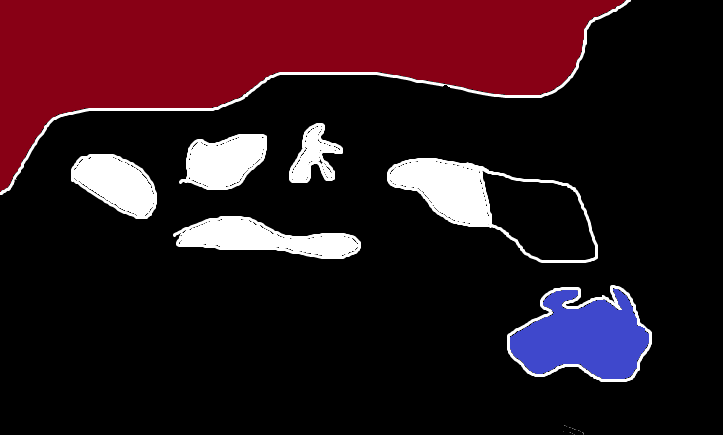
\includegraphics[scale=0.63]{indonesia-asia-australia}

Indonesia juga berada di antara Samudra \textbf{Hindia} dan \textbf{Pasifik}.

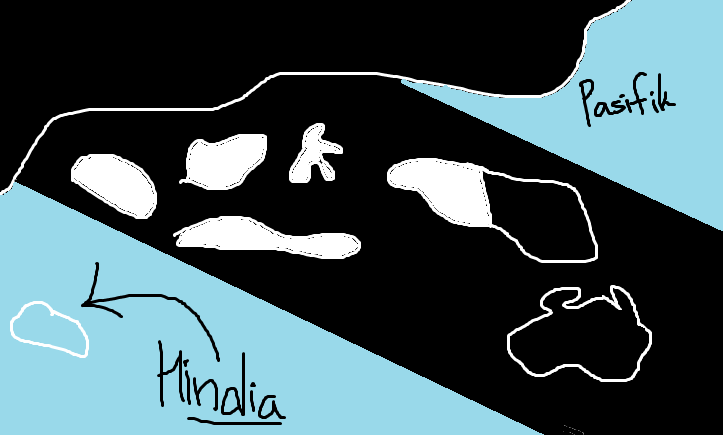
\includegraphics[scale=0.63]{indonesia-hindia-pasifik}

\end{document}
